% Für Bindekorrektur als optionales Argument "BCORfaktormitmaßeinheit", dann
% sieht auch Option "twoside" vernünftig aus
% Näheres zu "scrartcl" bzw. "scrreprt" und "scrbook" siehe KOMA-Skript Doku
\documentclass[12pt,a4paper,titlepage,headinclude,bibtotoc]{scrartcl}


%---- Allgemeine Layout Einstellungen ------------------------------------------

% Für Kopf und Fußzeilen, siehe auch KOMA-Skript Doku
\usepackage[komastyle]{scrpage2}
\pagestyle{scrheadings}
\setheadsepline{0.5pt}[\color{black}]
\automark[section]{chapter}


%Einstellungen für Figuren- und Tabellenbeschriftungen
\setkomafont{captionlabel}{\sffamily\bfseries}
\setcapindent{0em}


%---- Weitere Pakete -----------------------------------------------------------
% Die Pakete sind alle in der TeX Live Distribution enthalten. Wichtige Adressen
% www.ctan.org, www.dante.de

% Sprachunterstützung
\usepackage[ngerman]{babel}

% Benutzung von Umlauten direkt im Text
% entweder "latin1" oder "utf8"
\usepackage[utf8]{inputenc}

% Pakete mit Mathesymbolen und zur Beseitigung von Schwächen der Mathe-Umgebung
\usepackage{latexsym,exscale,stmaryrd,amssymb,amsmath}

% Weitere Symbole
\usepackage[nointegrals]{wasysym}
\usepackage{eurosym}

% Anderes Literaturverzeichnisformat
%\usepackage[square,sort&compress]{natbib}

% Für Farbe
\usepackage{color}

% Zur Graphikausgabe
%Beipiel: \includegraphics[width=\textwidth]{grafik.png}
\usepackage{graphicx}

% Text umfließt Graphiken und Tabellen
% Beispiel:
% \begin{wrapfigure}[Zeilenanzahl]{"l" oder "r"}{breite}
%   \centering
%   \includegraphics[width=...]{grafik}
%   \caption{Beschriftung} 
%   \label{fig:grafik}
% \end{wrapfigure}
\usepackage{wrapfig}

% Mehrere Abbildungen nebeneinander
% Beispiel:
% \begin{figure}[htb]
%   \centering
%   \subfigure[Beschriftung 1\label{fig:label1}]
%   {\includegraphics[width=0.49\textwidth]{grafik1}}
%   \hfill
%   \subfigure[Beschriftung 2\label{fig:label2}]
%   {\includegraphics[width=0.49\textwidth]{grafik2}}
%   \caption{Beschriftung allgemein}
%   \label{fig:label-gesamt}
% \end{figure}
\usepackage{subfigure}

% Caption neben Abbildung
% Beispiel:
% \sidecaptionvpos{figure}{"c" oder "t" oder "b"}
% \begin{SCfigure}[rel. Breite (normalerweise = 1)][hbt]
%   \centering
%   \includegraphics[width=0.5\textwidth]{grafik.png}
%   \caption{Beschreibung}
%   \label{fig:}
% \end{SCfigure}
\usepackage{sidecap}

% Befehl für "Entspricht"-Zeichen
\newcommand{\corresponds}{\ensuremath{\mathrel{\widehat{=}}}}
% Befehl für Errorfunction
\newcommand{\erf}[1]{\text{ erf}\ensuremath{\left( #1 \right)}}

%Fußnoten zwingend auf diese Seite setzen
\interfootnotelinepenalty=1000

%Für chemische Formeln (von www.dante.de)
%% Anpassung an LaTeX(2e) von Bernd Raichle
\makeatletter
\DeclareRobustCommand{\chemical}[1]{%
  {\(\m@th
   \edef\resetfontdimens{\noexpand\)%
       \fontdimen16\textfont2=\the\fontdimen16\textfont2
       \fontdimen17\textfont2=\the\fontdimen17\textfont2\relax}%
   \fontdimen16\textfont2=2.7pt \fontdimen17\textfont2=2.7pt
   \mathrm{#1}%
   \resetfontdimens}}
\makeatother

%Honecker-Kasten mit $$\shadowbox{$xxxx$}$$
\usepackage{fancybox}

%SI-Package
\usepackage{siunitx}

%keine Einrückung, wenn Latex doppelte Leerzeile
\parindent0pt

\usepackage{adjustbox}

%Bibliography \bibliography{literatur} und \cite{gerthsen}
%\usepackage{cite}
\usepackage{babelbib}
\selectbiblanguage{ngerman}

\begin{document}

\begin{titlepage}
\centering
\textsc{\Large Anfängerpraktikum der Fakultät für
  Physik,\\[1.5ex] Universität Göttingen}

\vspace*{3.5cm}

\rule{\textwidth}{1pt}\\[0.5cm]
{\huge \bfseries
  Versuch Dia- und Paramagnetismus\\[1.5ex]
  Protokoll}\\[0.5cm]
\rule{\textwidth}{1pt}

\vspace*{3.5cm}

\begin{Large}
\begin{tabular}{ll}
Praktikant: &  Michael Lohmann\\
 &  Felix Kurtz\\
% &  Kevin Lüdemann\\
% &  Skrollan Detzler\\
 E-Mail: & m.lohmann@stud.uni-goettingen.de\\
 &  felix.kurtz@stud.uni-goettingen.de\\
% &  kevin.luedemann@stud.uni-goettingen.de\\
% &  skrollan.detzler@stud.uni-goettingen.de\\
 Betreuer: & Björn Klaas \\
 Versuchsdatum: & 09.09.2014\\
\end{tabular}
\end{Large}

\vspace*{0.8cm}

\begin{Large}
\fbox{
  \begin{minipage}[t][2.5cm][t]{6cm} 
    Testat:
  \end{minipage}
}
\end{Large}

\end{titlepage}

\tableofcontents

\newpage

\section{Einleitung}
\label{sec:einleitung}
Magnetismus ist eine der wichtigsten Methoden, um elektrische Daten zu speichern.
So basieren herkömmliche Festplatten auf diesem Prinzip.
Um dies zu vermessen, kann man den zu untersuchenden Stoff in ein vorhandenes Magnetfeld führen und die Auswirkungen beobachten.

\section{Theorie}
\label{sec:theorie}
\subsection{Magnetfelder in Materie}
Die Ausbreitung von Magnetfeldern in Materie erfolgt nach den \textsc{Maxwell}-Gleichungen durch
\begin{align}
	\vec B&=\mu_0\vec H+\mu_0\vec M\approx\mu_0\mu_r\vec H
\end{align}
mit der magnetischen Suszeptibilität
\begin{align}
	\chi\vec M&=\vec H\\
	\Rightarrow\mu_r&=1+\chi .
\end{align}
$\mu _r$ nennt man auch die relative Permiabilität.
Dieser Zusammenhang gilt jedoch nach \cite[S. 112]{demtroeder2} nur für kleine magnetische Flussraten, da sonst $\vec M$ nicht mehr proportional zu $\vec H$ ist.

\subsection{Hallsonde}
Hallsonden funktionieren nach der Lorentzkraft.
Ein Strom wird durch ein Metallplättchen geleitet.
Ist dieses in einem Magnetfeld, so werden die Elektronen durch die Lorentzkraft abgelenkt.
Dadurch baut sich jedoch ein elektrisches Feld auf, was sie wieder zurück lenkt.
Durch den weiteren Weg steigt der Widerstand des durchflossenen Wegs.
Dieser kann nun vermessen werden und daraus kann der verlängerte Weg bestimmt werden und daraus widerum das Magnetfeld.

\subsection{Diamagnetismus}
Als diamagnetische Stoffe werden solche bezeichnet, welche eine aus einem äußeren Magnetfeld herausgedrängt werden.
Dies entsteht dadurch, dass sich in ihrem inneren Ströme bilden, welche nach der Lenzschen Regel der Ursache (dem Magnetfeld) entgegenwirkt. 
Solche Stoffen haben keine permanenten Dipole, da diese wieder Kräfte ausüben würden, welche deutlich stärker sind, als die diamagnetischen. 
Wie durch die Herkunft des Effektes zu erahnen, ist er kaum Temperaturabhängig.
Der Diamagnetismus tritt bei allen Metallen auf, wird aber häufig durch andere Effekte wie Ferro- oder Paramagnetismus überlagert.
Die bekanntesten Materialien mit diamagnetischen Eigenschaften sind Wasser, Kupfer, Gold oder Bismus (wie es in unserem Versuch verwendet wird).


\subsection{Paramagnetismus}
Der Paramagnetismus ist ein Effekt, bei dem in bestimmten Stoffen von außen angelegte Magnetfelder verstärkt werden.
Diese besteheh aus Atomen mit nicht vollständig gefüllten Elektronenschalen.
Ohne äußere Felder gleichen sich die magnetischen Momente, welche durch die nicht gleichmäßig verteilten Ladungen entstehen aus.
Wird jedoch ein externes Feld angelegt, so richten sich die Elementarmagnete an dem Feld aus.
Sie verstärken es so.
Mit steigender Temperatur werden die Elektronen jedoch immer weniger durch aüßere Felder beeinflusst, so dass dieser Effekt mit steigender Temperatur abnimmt.
Dies hat Marie \textsc{Curie} entdeckt und es in dem folgenden Gesetz beschrieben:
\begin{align*}
\chi=\frac{C}{T}
\end{align*}
mit der Materialkonstante $C$.

\subsection{Energie des magnetischen Feldes}
Nach \cite[S. 134]{demtroeder2} gilt für den Energiegehalt eines magnetischen Feldes
\begin{align*}
	W=-\int\frac{1}{2}\mu_0\mu_rH^2\cdot dV
\end{align*}
Ist das Feld im Inneren des Volumens annähernd konstant, so kann das Integral abgeschätzt werden durch
\begin{align}
	W\approx-\frac{1}{2}\mu_0\mu_rH^2\cdot V=-\frac{1}{2}\mu_0(1+\chi)H^2\cdot V=-\frac{1}{2}\mu_0H^2\cdot V-\frac{1}{2}\mu_0\chi H^2\cdot V\, .
\end{align}
was als Potential der Kraft aufgefasst werden kann.
Der erste Term gibt die Energie es Vakuums an und verschwindet bei der Gradientbildung.
Der zweite Teil ergibt im eindimensionalen Fall
\begin{align}
	F=-\nabla W=-\frac{\partial W}{\partial x}=-\frac{\chi V}{\mu_0}B\frac{\partial B}{\partial x}\, .\label{eq:GradW}
\end{align}

\section{Durchführung}
\label{sec:durchfuehrung}
Zunächst wird der Aufbau aus Abb. \ref{fig:schaltkreis} aufgebaut.
Dabei schaltet man eine Spule auf zwei Polschuhen über einen Schiebewiderstand mit einem Amperemeter in Reihe, wie in Abb. \ref{fig:schaltkreis} zu sehen.
%Da die Polschuhe nicht symmetrisch sind, sondern sich nach unten annähern, 

Zunächst wird der Widerstand so eingestellt, dass ein konstanter Strom von $1.2\si\ampere$ durch die Spulen fließt.
Ändert sich dieser, so ist der Widerstand nachzuregeln.
Das sich ergebende Magnetfeld wird nun mit der \textsc{Hall}sonde bestimmt.
Hierbei sollte die Schrittlänge 5mm nicht überschreiten.

Daraufhin wird die Position zwischen den Polschuhen vermerkt, wenn man die Körper an die Analysewaage hängt.
Anschließend werden die Massen der drei Probekörper (Ta, MnO$_2$ und Bi) aufgenommen, wie in Abb. \ref{fig:aufbau} zu erkennen ist.
Dies geschieht je für ein- und ausgeschaltetes Magnetfeld.
Diese Messungen werden je dreimal durchgeführt, wobei man zwischen den Messungen die Probekörper abnehmen oder zumindest anstoßen sollte.

Nun wird für die Position des Tantalkörpers und 5 und 10mm jeweils darüber und darunter das Magnetfeld für die Stromstärken ($0.8,\,1.0,\,1.2\text{ und }1.4\si\ampere$) vermessen.
Abschließend wird der Tantal-Körper erneut eingehängt und für die im letzten Schritt eingestellten Werte der Stromstärke werden jeweils drei Messungen der Gewichtskraft durchgeführt.
Auch hier ist der Körper zwischen den Messungen anzustoßen.



\begin{figure}[h]
	\centering
	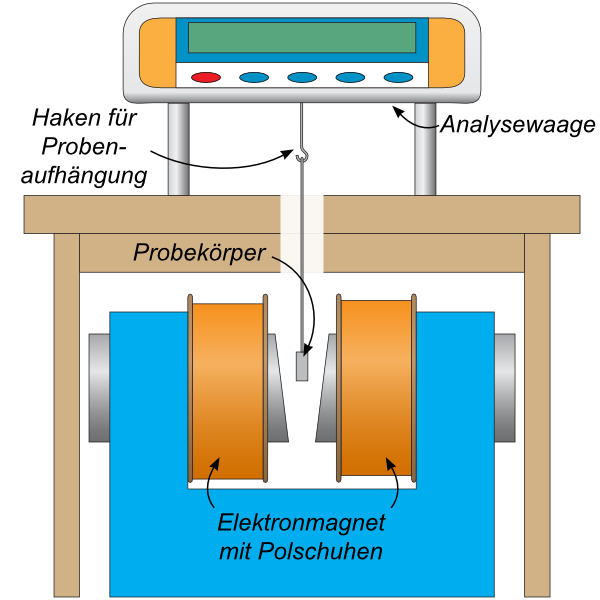
\includegraphics{aufbau}
	\caption{Aufbau der Waage zur Bestimmung der Kräfte nach \cite[15.11.14, 14 Uhr]{LP15}.}
	\label{fig:aufbau}
\end{figure}
\begin{figure}[h]
	\centering
	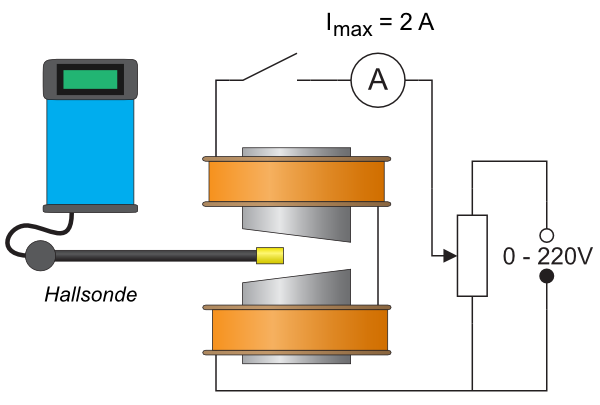
\includegraphics{schaltkreis}
	\caption{Schaltkreis zur Bestimmung von Dia- und Paramagnetismus nach \cite[15.11.14, 14 Uhr]{LP15}.}
	\label{fig:schaltkreis}
\end{figure}

\section{Auswertung}
\label{sec:auswertung}
\subsection{Ortsverlauf und Gradient $B$}
In Abb. \ref{fig:aus1} sind die Messwerte werden Messwerte der Flussdichte $B$ und der Gradient der Flussdichte gegen den Ort aufgetragen.
Hierbei kann man erkennen, dass zu Beginn das Magnetfeld stark steigt, bis es bei einer Höhe von 10mm das Maximum erreicht. danach fällt es fast linear ab.
Dies war auch zu erwarten, da die Polschuhe bei 10mm ihre geringste Entfernung hatten und danach sich linear voneinander entfernten.
Der Gradient bestätigt dies, da er im Maximum annähernd 0 ist und an höheren Orten ungefähr konstant ist.

Nach Gleichung \eqref{eq:GradW} gilt
\begin{align}
	F=-\frac{\chi V}{\mu_0}\cdot\frac{B\partial B}{\partial x}\, .\label{eq:FB}
\end{align}
In Abb. \ref{fig:aus3} ist genau $\frac{B\partial B}{\partial x}$ aufgetragen gegen die jeweilige Position.


\begin{figure}[h]
\centering
\adjustbox{width=0.8\linewidth}{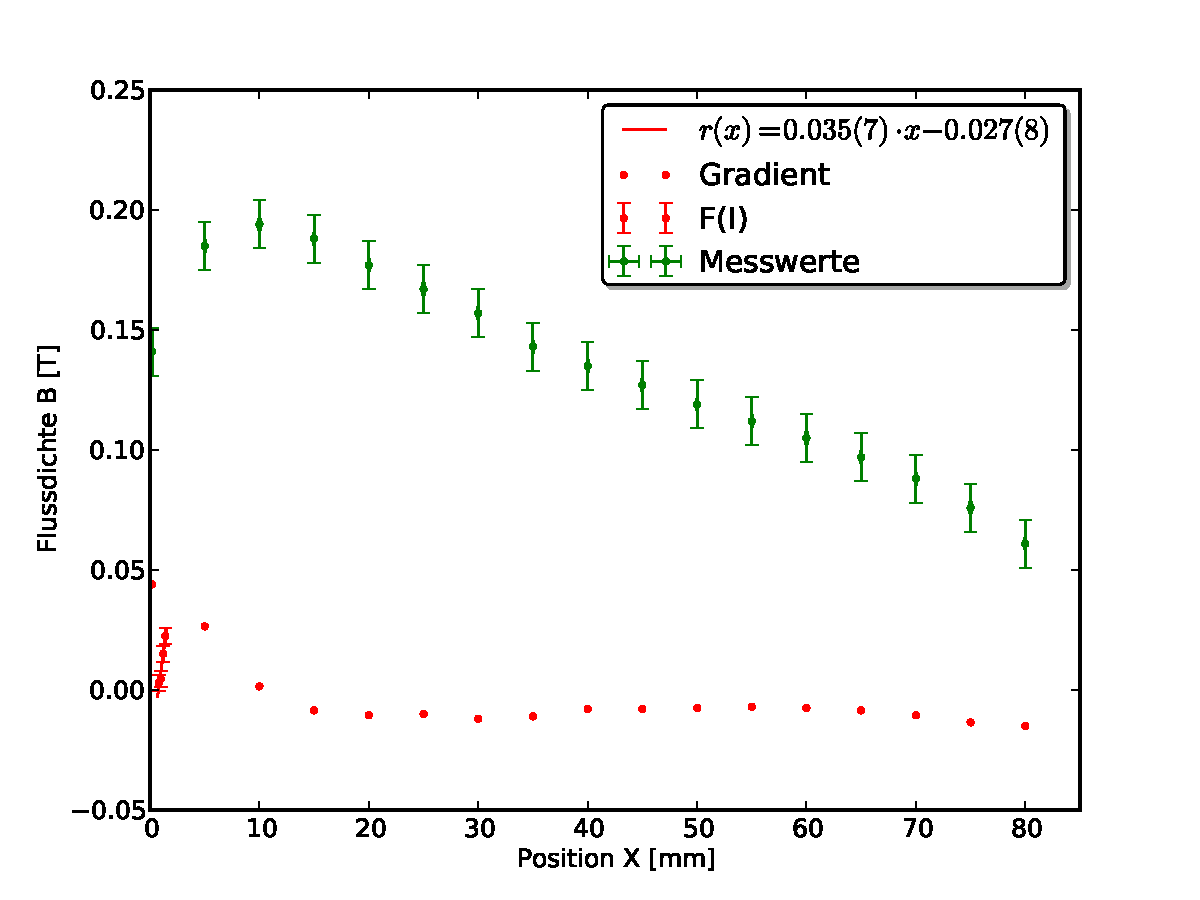
\includegraphics{Aus1}}
\caption{Auftragung der gemessenen Werte der Hallsonde zusammen mit der numerischen Ableitung aufgetragen gegen den Ort.}
\label{fig:aus1}
\end{figure}
\begin{figure}[h]
\centering
\adjustbox{width=0.8\linewidth}{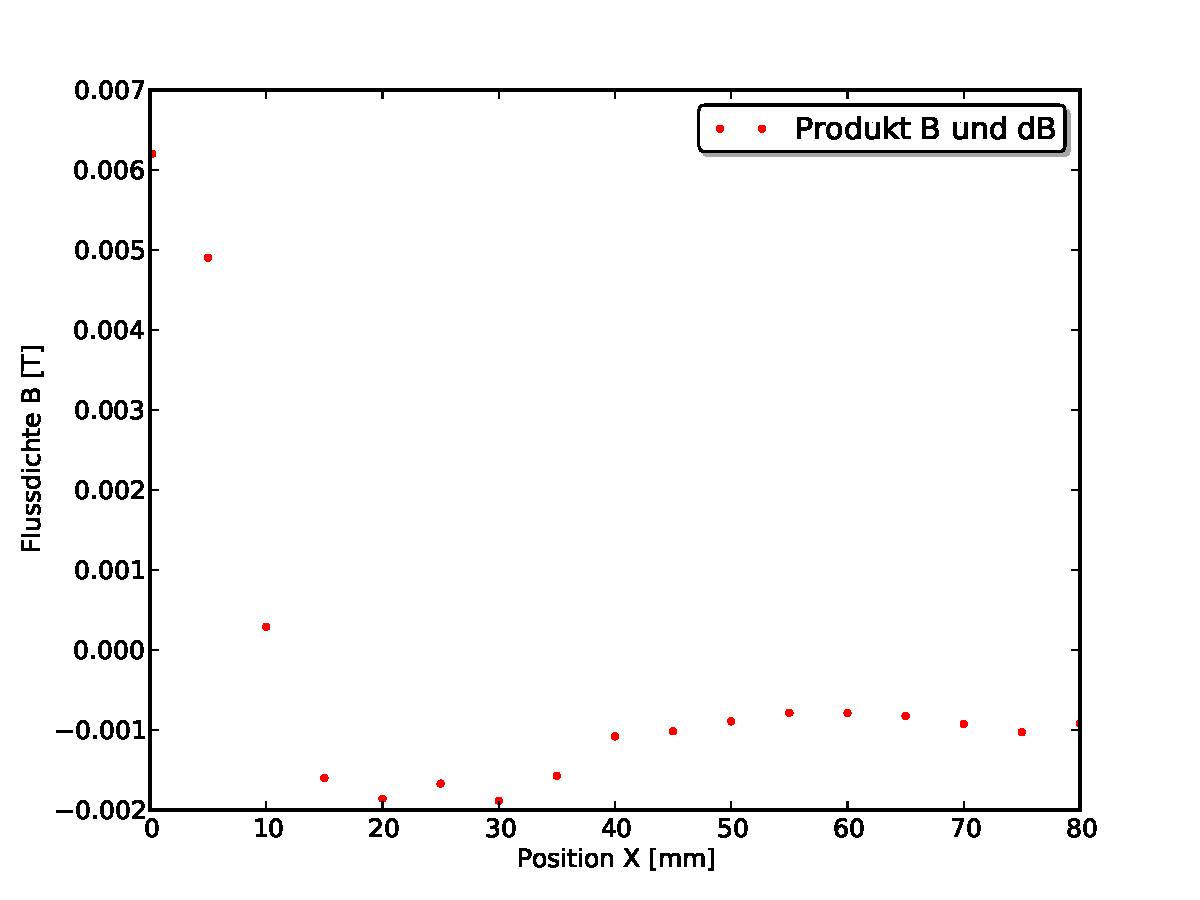
\includegraphics{Aus3}}
\caption{Produkt des $B$-Feldes mit der Ableitung an der jeweiligen Stelle.}
\label{fig:aus3}
\end{figure}

\subsection{Magnetische Suszeptibilität}
Nach Gleichung \eqref{eq:GradW} gilt 
\begin{align*}
	\chi=-\frac{V\cdot BB'}{\mu_0F}\, .
\end{align*}
Die durch das Magnetfeld ausgeübte Kraft $F$ berechnet sich nach
\begin{align}
	F=F_{g+\text{mag}}-F_g\, ,
\end{align}
wodurch sich $\chi$ berechnen lässt.
Die jeweils drei Messungen der Kräfte wurden mit der Standardabweichung berechnet.

Die Ergebnisse der spezifischen und magnetischen Suszeptibilitäten finden sich in Tabelle \ref{tab:suszep}.
Dabei berechnet sich $\chi_\text{spez}=\chi/\rho$ mit $\rho$ nach \cite{formelsammlung}.

\begin{table}
	\centering
	\begin{tabular}{|c|c|c|c|}
		\hline
		Stoff 	& Masse [g]	& spez. Suszept. $\chi_\text{spez}$ [$10^{-6}$]	& mag. Suszep. $\chi$ [$10^{-5}$] \\\hline\hline
		Ta	& 0.911		& $4.6\pm 0.8$ 			& $3.0 \pm 1.3$ \\\hline
		Mn	& 0.455		& $6.6 \pm 1.2$			& $1.0 \pm 0.4$ \\\hline
		Bi	& 0.851		& $-4.8 \pm 0.8 $		& $-1.3 \pm 0.6$\\\hline
	\end{tabular}
	\caption{Errechnete spezifische und magnetische Suszeptibilitäten der vermessenen Proben.}
	\label{tab:suszep}
\end{table}

Mit Werten für Ta bei $42.7$ mm: $B= 0.711$, $dB= -0.015$\\
Mn bei $49.4$ mm: $B= 0.762$, $dB= -0.007$\\
Bi bei $21.0$ mm: $B= 0.817$, $dB= -0.01$

\subsection{Flussdichte und Gradient verschiedener Stromstärken}
In Abbildung \ref{fig:aus61} sind die gemessenen Flussdichten an verschiedenen Orten für verschiedene Stromstärken verzeichnet.
Dabei fällt auf, dass die Flussdichte nahezu linear für eine Stromstärke verläuft und für eine größere höher wird, jedoch ihre Steigung nicht verändert.
Dies bedeutet, dass die Stromstärke zwar die Feldstärke, nicht jedoch den Verlauf des Feldes beeinflusst.

In Figur \ref{fig:aus62} ist der Gradient der Flussdichte für die obigen Messwerte eingetragen.
Dieser ist jedoch nicht linear fallend, sondern (z.B. für $I=1,2\si\ampere$ veringert er sich zuerst und steigt dann auf einen höheren Wert, als zu Beginn) folgt nur annähernd einer fallenden Geraden.


\begin{figure}[h]
\centering
\adjustbox{width=0.7\linewidth}{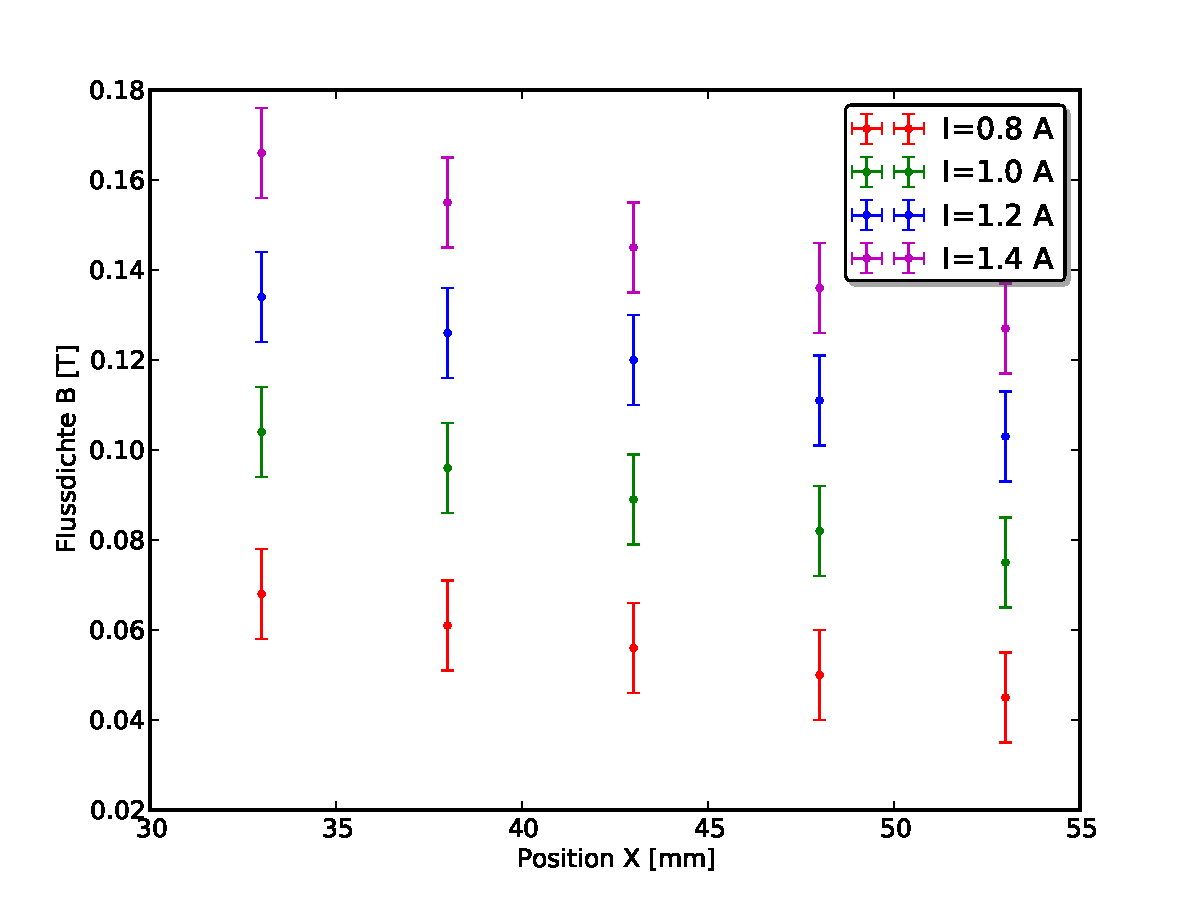
\includegraphics{Aus61}}
\caption{Gemessene Flussdichten $B$ für verschiedene Stromstärken.}
\label{fig:aus61}
\end{figure}
\begin{figure}[h]
\centering
\adjustbox{width=0.7\linewidth}{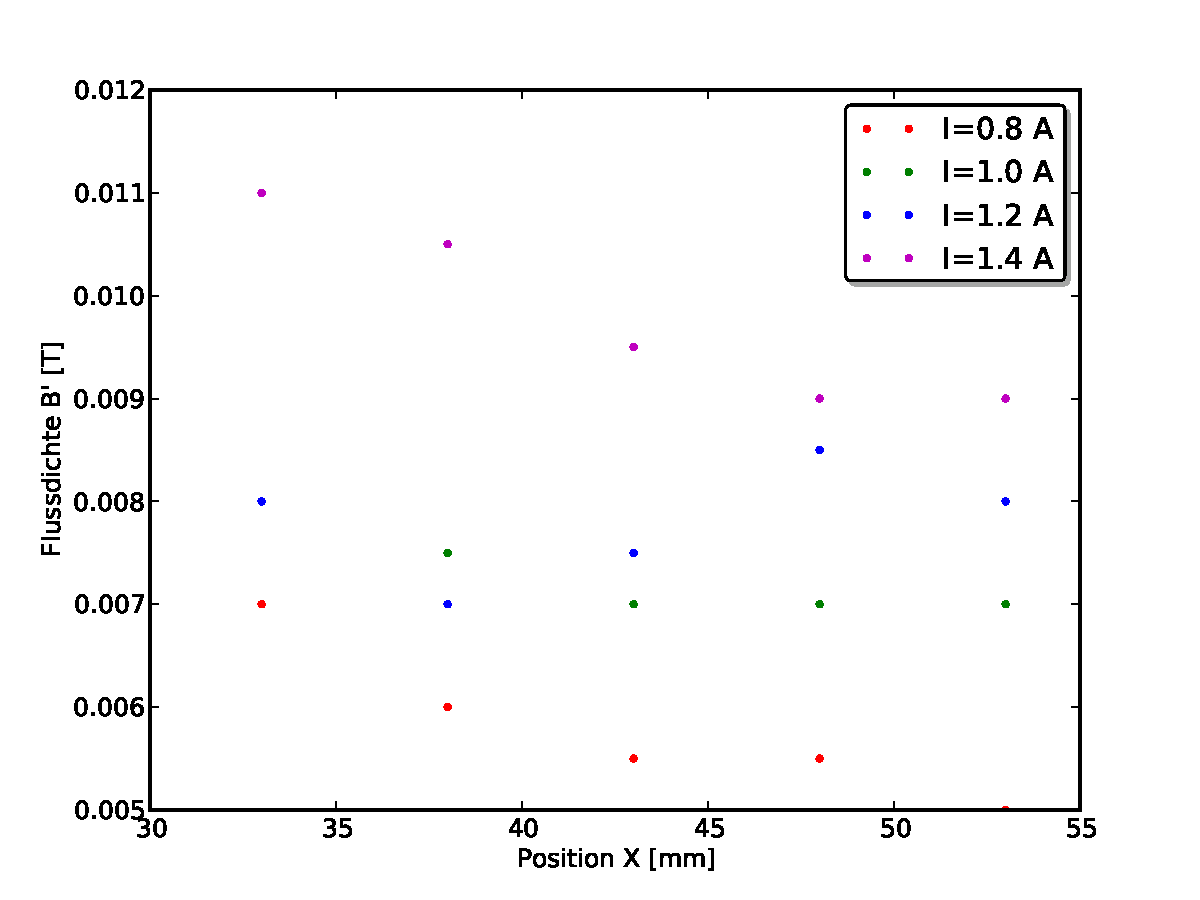
\includegraphics{Aus62}}
\caption{Gradient $B'$ der Flussdichte für verschiedene Stromstärken.}
\label{fig:aus62}
\end{figure}
\subsection{Kraft auf Tantal}
Nach der umgestellten Gleichung \eqref{eq:FB} gilt
\begin{align*}
	B=\frac{\mu_0F}{\chi VB'}\, .
\end{align*}
Die in Abbildung \ref{fig:aus7} aufgetragene gemessene Kraft auf den Tantal-Probekörper zeigt einen linearen Zusammenhang bezüglich der Stromstärke.
Das reduzierte $\chi^2$ des linearen Fits beträgt 0.75 und bestätigt damit diesen optischen Eindruck.



\begin{figure}[h]
\centering
\adjustbox{width=0.8\linewidth}{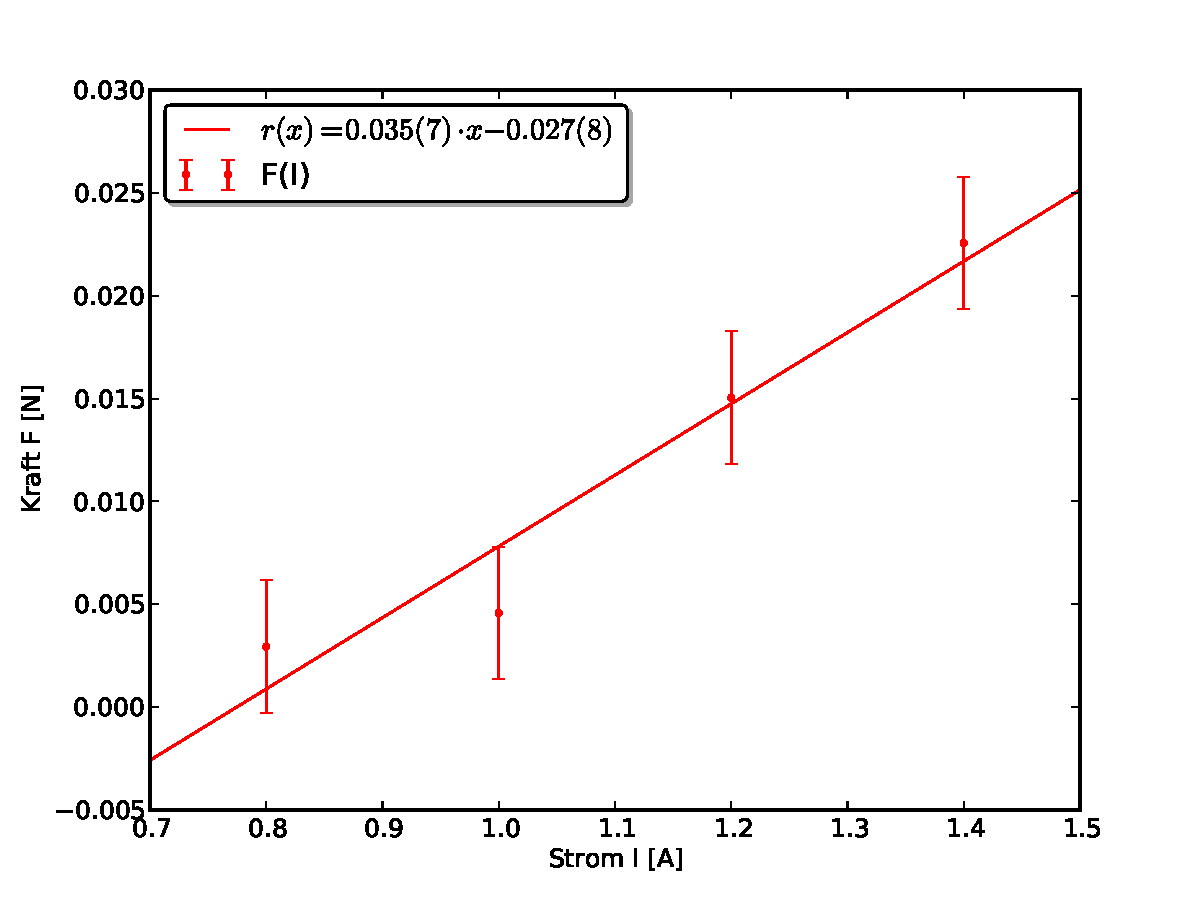
\includegraphics{Aus7}}
\caption{Gemessene Kraft auf den Tantal-Probekörper bei verschiedenen Stromstärken zusammen mit der linearen Regression.}
\label{fig:aus7}
\end{figure}

\section{Diskussion}
\label{sec:diskussion}
In Abb. \ref{fig:aus3} fällt auf, dass die wirkende Kraft (welche nach Gleichung \eqref{eq:GradW} proportional zu $BB'$ ist) nach 30mm wieder ansteigt.
Dies ist möglicherweise darurch zu erklären, dass das Magnetfeld nicht homogen abnimmt, sondern Störungen besitzt.

Den wohl größten Störeinfluss auf alle Messungen mit der Hallsonde hatte vermutlich der Offset der Hallsonde.
Dieser schwankte zwischen -0.55 und -0.77T.
Dies lässt keine qualifizierten Erkenntnisse der Messung zu, da die Messwerte weniger als 0.9T und somit die Schwankungen 30\% der Messwerte betrugen.\\
Durch dies werden die Ergebnisse verfälscht.\\

Die Testkörper hingen bei den Messungen meistens nicht still, da kleine Luftbewegungen die Massen immer wieder in Schwingungen versetzen.
Die Analysewaage besitzt für Messungen auf der Waagfläche ein Glaskasten, der dies verhindern soll, jedoch werden bei unseren Messungen die Massen unten angehängt.\\

Die Literaturwerte aus verschiedenen Büchern (z.B. \cite{gerthsen} und \cite{taschenbuch}) stimmen nicht überein.
Jedoch sind auch die Größenordnungen der Messungen nicht korrekt.
\newpage
\bibliography{literatur}
\bibliographystyle{babalpha}
\end{document}
